\chapter{Introduction (draft)}
\label{ch:intro}

\section{Obesity}
\label{sec:obesity}

Obesity has been one of the major global problems for more than a decade, associated with many noncommunicable diseases such as diabetes, cardiovascular diseases and certain types of cancers \citep{WHO2014}.
In fact, the risk of comorbidities increases with the increase in \gls{bmi}, where the risk becomes severe as the \gls{bmi} level approaches the obese category \citep{WHO2000}.

The number of overweight and obese people, in both adults and children, have risen in every country of the world, and the trend continues as we speak.
Estimated to account for 3.4 million deaths per year and 93.6 million \glspl{daly} in 2010, obesity is a serious disease that continues to grow in our society \citep{Lim2012}.

\subsection{Definition of obesity}
\label{sub:definition_of_obesity}

Obesity is defined as an abnormal or excessive fat accumulation that may impair health of that individual \citep{Garrow1988}.

One common and widely used approach to categorise individuals is by measuring the \gls{bmi} of the individual.
\gls{bmi} is a measurement based on the weight-to-height ratio of an individual that is used by clinicians and epidemiologists to classify adults into underweight, normal weight, overweight or obese categories.
The unit of \gls{bmi} is defined as the individual's weight in kilograms per square of the height in meters (kg/m$^2$).

\gls{who} (2014) have used \gls{bmi} measurements to define overweight and obesity in adults as an individual with \gls{bmi} $\geq$ 25 kg/m$^2$ and $\geq$ 30 kg/m$^2$, respectively.
For children under the age of 5, overweight and obesity were defined as weight-for-height greater than 2 standard deviation and 3 standard deviation above \gls{who} Child Growth Standards median, respectively.
For children aged between 5 to 19 years, overweight and obesity were defined as BMI-for-age greater than 1 standard deviation and 2 standard deviation above \gls{who} Growth Reference Standards median, respectively.

Although the use of \gls{bmi} as an accurate measure of body fat composition and/or representation of the individual's metabolic status remains controversial, many studies have used \gls{bmi} due to the ease of data collection compared to other measurements, such as waist-to-height ratio \citep{Lee2008, Gelber2008}.
Consequently, most of the publicly available clinical data have height and weight data from which one can calculate the patients' \gls{bmi}, and therefore able to collect the patients' obesity status more conveniently than, for example, waist-to-height ratio.

\subsection{Prevalence of obesity}
\label{sub:prevalence_of_obesity}

From the latest global status report on noncommunicable diseases by \citet{WHO2014}:
\begin{quote}
	\textit{
		In 2014, 39\% of adults aged 18 years and older (38\% of men and 40\% of women) were overweight.
		The worldwide prevalence of obesity nearly doubled between 1980 and 2014.
		In 2014, 11\% of men and 15\% of women worldwide were obese.
		Thus, more than half a billion adults worldwide are classed as obese.
	}
\end{quote}

\noindent
This equated to approximately 1 in every 14 people in the world classed as obese in 2014, and therefore, 1 in 14 people around the world were also at severe health risks associated with obesity.
It was also noted in the report that women were more likely to be obese than men, and that the prevalence of overweight and obesity increased as the income level of the countries increased \citep{WHO2014}.

In addition to this, the worldwide prevalence of childhood overweight and obesity has been increasing steadily since 2000 \citep{WHO2014}.
Furthermore, the prevalence of overweight in children under 5 years was estimated to reach from 6.3\% in 2013 to 11\% by 2025 if the current trend continued \citep{WHO2014}.
The current obesity status of the adult population is bad already, but the fact that more of the younger population who are overweight and obese poses a much greater risk for the health of the population (discussed in \cref{sub:impact_of_obesity}).

% TODO: Add western-specific and NZ specific statistics on obesity
% TODO: Add male/female specific stats
% TODO: Add Maori/PI specific stats

Until these terrible trends stop, and even after the trends stop, the world will need a plan to live along with this ongoing global epidemic of obesity and its associated diseases.

\subsection{Physiological mechanism of obesity}
\label{sub:physiological_mechanism_of_obesity}

Obesity is caused by continuous intake of food, whether they are controlled or not, without expending all of the energy gained.
The key to the problem is the control of food intake and energy expenditure, and how they are regulated in your body.

\subsubsection{Role of hypothalamus and arcuate nucleus in food intake control}
\label{ssub:role_of_hypothalamus_and_arcuate_nucleus_in_food_intake_control}

The central role of hypothalamus in the context of obesity is the control of satiety, and therefore food intake.
The hypothalamus receives both nueronal and hormonal inputs from the body and propagates the signal to the downstream neurons that ultimately affect the food intake of the individual \citep{Bell2005, Spiegelman2001}.

Within the hypothalamus, there is a group of neurons located within the arcuate nucleus that is essential for satiety signal transmission.
There are two types of neurons in the arcuate nucleus: orexogenic and anorexogenic neurons.
Orexogenic neurons are responsible for the promotion of food intake and reducing energy expenditure, whereas the anorexogenic neurons have the opposite effect \citep{Barsh2002}.

The orexogenic neurons produce \gls{npy} and \gls{agrp} which induces orexogenic signal to the downstream neurons; anorexogenic neurons produce \gls{pomc} and \gls{cart} which induces anorexogenic signal to the downstream neurons \citep{Barsh2002, Spiegelman2001}.
When stimulated by, for example, endocrine signals, these two different types of neurons act on the downstream neurons to promote or reduce food intake and energy expenditure.

\subsubsection{Leptin-melanocortin pathway}
\label{ssub:leptin_melanocortin_pathway}

Leptin-melanocortin pathway is the pathway in which the level of satiety is controlled and regulated.
In this pathway, both the orexogenic and anorexogenic neurons have crucial roles in controlling the satiety of the individual, and therefore their eating behaviour.

When a satiety-controlling hormone such as leptin reaches the arcuate nucleus region of the hypothalamus, it can stimulate or inhibit orexogenic, anorexogenic, or both orexogenic and anorexogenic neurons.
Depending on which neurons are stimulated or inhibited, the hormone will ultimately alter the satiety level of the individual.\\

\noindent
Both \gls{pomc} and \gls{cart} are strong anorexogenic neuropeptides that stimulate the downstream effector neurons via the \gls{mc4r} pathway \citep{Barsh2002}.

\gls{pomc} is a precursor protein that is cleaved to produce \gls{acth}, $\alpha$-, $\beta$- and $\gamma$-\gls{msh}, and $\beta$-endorphin \citep{Smith1988}.
Perhaps the most important, or most relevant, in the context of obesity and satiety control is the $\alpha$-MSH.
$\alpha$-MSH is the main ligand that binds to the \gls{mc4r} expressed in the brain, and sends anorexogenic signals to the downstream neurons through this pathway \citep{Krude1998}.

Similarly, \gls{cart} is also a neuropeptide that has a strong anorexogenic effect discovered by \citet{Kristensen1998}.
Unlike $\alpha$-MSH, the receptor for \gls{cart} has not been identified yet, and the exact mechanism in which \gls{cart} acts is unclear \citep{Kristensen1998, Rogge2008}.

Since the expression of both neuropeptides are under the control of leptin, and that $\alpha$-MSH is known to stimulate the melanocortin pathway to produce an anorexogenic signal to the downstream neurons, this satiety-controlling signalling pathway is known as the leptin-melanocortin pathway.
\\

\noindent
In contrast to the \gls{pomc}/\gls{cart} neurons, orexogenic neuropeptides \gls{npy} and \gls{agrp} are produced in the \gls{npy}/\gls{agrp} neurons when stimulated by hormones that control satiety.

\gls{npy} was first discovered by \citet{Tatemoto1982}, and later associated with altered eating behaviour in rats by \citet{Clark1984}.
\gls{npy} is recognised by the \gls{nyr1}, a G protein-coupled receptor expressed on the downstream effector neurons, which relays the orexogenic signal from the \gls{npy}/\gls{agrp} neurons \citep{Barsh2002, Bell2005, Herzog1992}

Agouti protein is a protein normally expressed in the skin where it affects the pigmentation, and was first identified over 100 years ago by \citet{Castle1910} in mice that had yellow, or agouti-coloured coat.
Although the fact that ubiquitous expression of agouti protein caused obesity in mice was known for a long time, the biochemical mechanism that caused such phenotype was not elucidated until 1997 by \citet{Ollmann1997}.
In brief, \gls{agrp} was shown to be a strong antagonist of the \gls{mc4r}, expressed in the downstream neurons to the \gls{npy}/\gls{agrp} neurons, and thus inhibited the anorexogenic signalling through the melanocortin pathway \citep{Barsh2002,Ollmann1997}.\\

\noindent
Together, \gls{npy}/\gls{agrp} and \gls{pomc}/\gls{cart} neurons produce contrasting signals that affect the overall satiety of the individual.
Depending on how strong or weak these signals are, the individual may be more or less susceptible to obesity.

\subsubsection{Role of hormones in leptin-melanocortin pathway}
\label{ssub:role_of_hormones_in_leptin_melanocortin_pathway}

There are many hormones in your body that regulates various physiological aspects of your body.
Out of the many, four hormones in particular have an important role in regulating the satiety of an individual: ghrelin, leptin, insulin, and \gls{pyy}.\\

\noindent
Ghrelin, originally identified as a peptide that stimulated the release of growth hormone from the pituitary, is a hormone produced mainly in the stomach that has a significant role in meal initiation and food intake, as well as energy homeostasis \citep{Kohno2003, Kojima1999, Nakazato2001}.
Ghrelin is known to be a ligand for the \gls{ghsr} which is expressed abundantly on the \gls{npy}/\gls{agrp} neurons, and increases the Ca$^{2+}$ concentration in these neurons \citep{Kohno2003}.

Furthermore, \citet{Seoane2003} showed that ghrelin increased the mRNA levels of both \gls{npy} and \gls{agrp} in these neurons and hence their protein expression, indicating the role of ghrelin as the orexogenic hormone that affects the overall outcome of the satiety signal.
\\

\noindent
Leptin, on the other hand, is a hormone that has an opposite effect as ghrelin, where the hormone signals satiety and reduces food intake.
First identified by \citet{Zhang1994}, the dicovery of the leptin gene, followed by the discovery of leptin receptor gene by \citet{Tartaglia1995}, were probably the major breakthrough in the field of obesity research.

Leptin is produced and secreted mainly by the white adipose tissue, and the circulating concentration of leptin in the body is proportional to body fat stores \citep{Barsh2002, Moustafa2013, Zhang1994}.
Leptin receptor has many splice variants, but the long variant of the leptin receptor is highly expressed only in the hypothalamus \citep{Ghilardi1996, Lee1996}.
In addition to this, leptin receptor is expressed on both the \gls{npy}/\gls{agrp} and \gls{pomc}/\gls{cart} neurons, and have different effect on the outcome of the satiety signal depending on which neuron leptin stimulates.

In \gls{npy}/\gls{agrp} neuron, it has been shown to reduce the Ca$^{2+}$ concentration, antagonising the effect of ghrelin on this type of neurons \citep{Kohno2003}.
Furthermore, binding of leptin to the leptin receptor on the \gls{npy}/\gls{agrp} neuron causes a decreased release of \gls{gaba}, which inhibits the \gls{pomc}/\gls{cart} neuron \citep{Cowley2001}.

In \gls{pomc}/\gls{cart} neuron, binding of leptin to its recpetor causes a depolarisation of the neuron \citep{Cowley2001}.
Together with the indirect effect from the \gls{npy}/\gls{agrp} neuron, leptin promotes the \gls{pomc}/\gls{cart} neuron to release $\alpha$-\gls{msh}, and therefore sends a anorexogenic signal to its downstream effector neurons.
\\

\noindent
Insulin, perhaps the most well-known hormone for its role in glucose homeostasis, also has an important role in satiety and food intake regulation.

Briefly, when insulin binds to the insulin receptor, \gls{irs} protein family is recruited and phosphorylated by the insulin receptor's intrinsic tyrosine kinase activity \citep{Saltiel2002}.
The phosphorylated \gls{irs} protein then activates \gls{pi3k}, which in turn activates its downstream targets, causing a rapid signal cascade through the cell \citep{Saltiel2002}.

The evidence of insulin's involvement in the satiety control was not particularly clear; even though there were strong evidence of obesity with neuron-specific deletion of insulin receptor, and that the insulin level, like leptin, was proportional to the fat mass also suggested the role of insulin in satiety and body weight control \citep{Barsh2002, Bruning2000, Woods1979}.
This was perhaps due to the fact that leptin and insulin used two different signalling pathways in the cell: leptin used the \gls{jak}/\gls{stat} signalling pathway, whereas insulin used the \gls{pi3k} pathway for signalling \citep{Ghilardi1996}.
This was puzzling to the researchers as there seemed to be no converging point of the two hromones in these pathways.

However, leptin, and subsequently insulin, was shown to activate ATP-dep\-endent K$^+$ channel in glucose-responsive neurons in the hypothalamus \citep{Spanswick1997, Spanswick2000}.
The activation of K$^+$ channel provided evidence for the two pathways to act similarly on the cell, at least for an acute response, suggesting a convergence in the pathway response by the two hormones, and therefore their role in satiety control.
\\

\noindent
The last hormone is the \gls{pyy}, a peptide hormone released by the distal gastrointestinal tract that produces an anorexogenic signal.

\gls{pyy} is a gut hormone that is secreted postprandially, and it is released at levels proportional to the calorie content of the meal \citep{Adrian1985}.
\gls{y2r} is an inhibitory presynaptic receptor that is highly expressed in the \gls{npy}/\gls{agrp} neuron, and is the target of the \gls{pyy} hormone \citep{Batterham2002}.
\citet{Batterham2002} showed that \gls{pyy} decreased the expression of \gls{npy} in the \gls{npy}/\gls{agrp} neuron, and activated the \gls{pomc}/\gls{cart} neuron by membrane depolarisation.
The two mechanisms of \gls{pyy} produces an anorexogenic signal and encourages the individual to stop eating.\\

\noindent
When any one of these neurons, neuropeptides, hormones or its corresponding receptors become defective, it can lead to some form of eating disorder (briefly covered in \cref{ssub:Individual-level_(micro-level)_factors}: \nameref{ssub:Individual-level_(micro-level)_factors}).
Therefore the roles of these neurons, neuropeptides, and hormones are crucial for healthy diet and body weight maintenance.

\subsection{Factors that affect the prevalence of obesity}
\label{sub:factors_that_affect_the_prevalence_of_obesity}

As one can suspect, there are many factors involved with the likelihood of an individual to become overweight and obese.

\subsubsection{Individual-level (micro-level) factors}
\label{ssub:Individual-level_(micro-level)_factors}

There are many environmental factors associated with the global rise in obesity (discussed in \cref{ssub:Population-level_(macro-level)_factors}: \nameref{ssub:Population-level_(macro-level)_factors}).
Even though these environmental factors are probably the most significant contributor of the current global obesity epidemic, there are some individual-level, genetic factors that assist in the overall increase in the proportion of the population that are obese.

There are many evidence of obesity being caused by individual-level genetic factors that make some individuals more predisposed to obesity than others.
Generally speaking, there are two classes of genetically-driven obesity: monogenic obesity and polygenic obesity \citep{Moustafa2013}. \\

\noindent
Monogenic obesity is where a single mutation in one of the genes that is directly involved in the obesity pathway causes severe obesity in the individual.
Since these mutations are usually directly related to the key neurons/neuropeptides/hor\-mones that were mentioned earlier (\cref{sub:physiological_mechanism_of_obesity}), the resulting phenotype from the mutation causes severe early-onset obesity.
However, although these mutations cause a devastating effect on the individual, these mutations occur very rarely in the population.
With that said though, the identification of these mutations have shed light on the mechanisms in which obesity is developed and it is worth mentioning some of these mutations to highlight the importance of the components involved in the obesity pathway.

The first mutation that should be mentioned is in the leptin gene.
\citet{Montague1997} found a single nucleotide deletion mutation at position 133 of the leptin gene in children with early-onset obesity.
They further showed that the mutation caused a frameshift mutation in the protein, resulting in an inactive form of leptin that was not able to be secreted \citep{Montague1997}.

In close relation to this mutation is the mutation in the leptin receptor gene.
\citet{Clement1998} have discovered a single nucleotide substitution mutation that led to the leptin receptor transcript that skipped exon 16, leading to a form of the receptor with no transmembrane or intracellular domain.
Individuals with this rare mutation showed extreme hyperphagia and symptoms of early-onset obesity, even though their circulating leptin levels were present abundantly \citep{Clement1998}.

The next couple of mutations are associated with the synthesis and the processing of \gls{pomc}.
\citet{Krude1998} found single nucleotide mutations in the exonic region of the \gls{pomc} gene that affected the transcription of the $\alpha$-\gls{msh} region (and some other regions) of \gls{pomc}.
\citet{Jackson1997} identified a mutation in the \gls{pc1}, an enzyme responsible for the processing of many prohormones and neuropeptides, including \gls{pomc}.
In either case, the mutation resulted in the lack of $\alpha$-\gls{msh} in the neurons for satiety signalling and caused severe early-onset obesity.

As mentioned earlier, even though these mutations are very rare and affects only those individuals that have one of these mutations, it had a profound impact in the field of obesity research and contributed significantly to the knowledge of the mechanism of how obesity develops.
\\

% \citep{Farooqi2003}
% \citep{Kublaoui2006}
% \citep{Dubern2001}
% \citep{Challis2002}
% \\

\noindent
Polygenic obesity is where a combination of variants in multiple genes or multiple regions of the genome, together with environmental factors, causes obesity in the individual \citep{Moustafa2013}.
Unlike in monogenic obesity where a single mutation in a gene causes severe obesity, the variants in some of the genes or genomic regions involved in polygenic obesity have little effect on the individual's obesity status by itself, but in combination with many other variants, together with environmental factors, it has a serious effect on the individual.

Known as the ``thrifty gene'' hypothesis, \citet{Neel1962} suggested that the genes that were important in obesity have been around in the population for many generations, as it would have had a selective advantage in an environment where the population experienced starvation more frequently than the current generation.
However, as food became more accessible, a subset of the population who were particularly good at storing fat and survive the starvation period ``overreacted'' to this rapid change in the environment \citep{Bell2005, Spiegelman2001}.
These observations in the rise in obesity in subsets of population cannot be explained simply by external factors alone, and there is a significant genetic component involved in this phenomenon \citep{Bell2005}.

There have been many studies that have investigated the association of genes and/or genomic regions with obesity.
Of those, many of the \glspl{gwas} published in 2007 that showed strong evidence of the \gls{fto} gene with \gls{bmi} and obesity were of greatest significance \citep{Dina2007,Frayling2007,Gerken2007,Scuteri2007}.
Until these studies came out, there has been no common genes or genomic regions that associated with obesity that was reproducible and reliable \citep{Frayling2007}.
Thus, these studies were the first evidence of common variants that contributed to the polygenic obesity phenotype in the population.

Discovery of the \gls{fto} gene has lead to extensive research on the gene, and the mechanism of action by the \gls{fto} variant has been recently uncovered  from these efforts \citep{Claussnitzer2015a,Smemo2014a}.
The association between obesity and genetic variations, and their mechanisms that lead to obesity, has not been fully elucidated due to its complexity, but it may not be long before they are fully uncovered.


\subsubsection{Population-level (macro-level) factors}
\label{ssub:Population-level_(macro-level)_factors}

Even though some individual-level factors are involved with obesity, it is clear that these individual-level factors cannot be accounted for the global epidemic of obesity that the world currently observes.
For this reason, obesity is thought to be caused mainly by the environmental factors that are present in the population.\\

\noindent
The first key factor that contirbutes to the global rise in the proportion of the population that is obese is the availability and abundance of certain food in the country.
With the help from government trade policies, food and other goods have become easier to trade between the country, helping the economic growth of many countries around the world \citep{Kearney2010}.
This led to greater abundance of food in general, greater number of choices of food and shifted the overall nutritional status of the country \citep{Malik2013}.
This shift in the food choice and availability (and the economic benefit associated with the trades) had a positive impact on the country, but the growth in the food market also resulted in a different, much larger problem -- obesity.

As an example, in the \gls{usa}, the cost of corn and soy is low due to the fact that they are the raw ingredients for most processed food and beverages, such as high fructose corn syrups used to sweeten many soft drinks in the \gls{usa} \citep{Malik2013}.
Moreover, corn and soy are also the main food for the livestock, which results in lower prices for meat \citep{Malik2013}.
On the othere hand, the prices of fruits and vegetables remain expensive due to the lack of support by the government to lower the cost associated with the production \citep{Malik2013}.

As a result, more people are inclined to consume food that are cheap, have little nutritional value and high in energy, than the food that are expensive, nutritional and healthy alternatives.
Thus, the population is more likely to become obese by making worst food choice.\\

\noindent
The second factor to consider is the behavioural changes led by the urbanisation of the population.
Urbanisation is defined as the gradual increase in the proportion of people living in urban areas.
As more people take up urban lifestyle, they are exposed to the new environment where there is a better range of food selection, as well as technological and mechanical advancement in transport and other daily chores that may not be available in rural areas where these people come from.

Although there are many advantages involved with urbanisation, such as access to developed health care systems, education and advanced technologies, the lifestyle change also impose negative health behaviour that ultimately lead to positive energy balance and therefore obesity \citep{Malik2013}.

Lack of physical activity is one of the obvious components that contribute to obesity, which is also linked with the urbanisation of the population.
Currently, the recommended amount of physical activity to keep an individual fit and healthy is $\geq$ 150 min of moderate-intensity aerobic physical activity per week, or $\geq$ 30 min of physical activity on most days of the week \citep{Pate1995, WHO2010}.
However, in many urban cities, this recommended level of physical exercise is difficult to achieve and maintain, due to the shift towards the sedentary behaviours that are encouraged by the developed transport system, automated household chores, and indoor entertainment \citep{Malik2013}.

Urbanisation by itself cannot be accounted for the lack of exercise in the population, but it is true that urbanisation makes the bar higher for many people to take up the recommended level of fitness and maintain it. \\

\noindent
The third factor is the income and socioeconomic status of the population.
As the average income increases, more people are able to buy food and are likely to take up the sedentary lifestyle.
Clearly, these behavioural changes will increase the likelihood of becoming obese.

From this, one would expect the high-income group to have the largest impact from obesity, but on the contrary to this expectation, the biggest impact from obesity is seen in the low- and middle-income groups of the population \citep{Malik2013}.
As mentioned briefly earlier, access to the developed health care system will allow weight maintenance of the population, but this is likely to be of most benefit for the high-income group in the population.
The reason for this is, quite simply, the cost associated with the visit to the health care system, and therefore high-income group is more likely to make a consistent and periodic visit than the low or middle-income group of the population \citep{Malik2013}.

So, for the low- and middle-income groups, the rise in average income in these groups allow the people to have access to food and activities that promotes sedentary bahaviours, but the limited access to the health care system, education and recreational activities that promote physical activites ultimately leads to positive energy balance and obesity \citep{Malik2013}.
In contrast, the high-income group of the population have better access to the facilities that promote weight maintenance, thus have less of an impact from obesity compared with the low- and middle-income groups of the population.\\

\noindent
The last factor, which ties in strongly with the first key factor, is the choice of diet made by the population.
The amount of low-quality food have increased significantly in many rapidly growing countries, as these high-energy, low-nutritional food are cheaper and more profitible than the natural produce that have higher nutritional value \citep{Kearney2010}.
As a result, more people tend to purchase these low-quality food more often, and consume more energy than they are required.

However, many people eat responsibly and avoid these low-quality diet and prevent overconsumption of such food, but the overconsumption of these food is not a big problem as such, rather the overall quality of the food \citep{Malik2013}.
These food are usually high in refined sugar and unhealthy fat, highly processed, contain very little nutritional value and are low in fibre.
As a result, consumption of these food increases the overall energy intake and achieve no nutritional benefits from the food.

Whether it is by choice or not, consumption of these low-quality diet leads to obesity and obesity-related diseases. \\

\noindent
All of these population-level environmental factors in synergy with the individual-level genetic factors have contributed to the global epidemic of obesity.

\subsection{Impact of obesity}
\label{sub:impact_of_obesity}

As mentioned at the beginning of the current section, obesity has a devastating effect on the health of the population in a global scale.

Overweight and obesity have been a risk factor for many diseases, including type 2 diabetes, cardiovascular diseases, hypertension, and many types of cancers \citep{Franks2010, Guh2009, Yach2006}.
As \citet{Yach2006} mentions in their paper, ``overweight and obesity have become to diabetes what tobacco is to lung cancer'', and it is important to understand that obesity has significant risks and comorbidities associated with it.

Although adulthood obesity is clinically important for risk assessment of diseases, childhood obesity has been focussed more heavily in recent years,  as it has greater public health implications.
There are many immediate consequences that are related to childhood obesity, but the diseases that develop as these children grow up are more critical than the earlier effects.

In the paper written by \citet{Must1999}, they reviewed many of the clinical studies done in the 1900s and summarised the risks associated with childhood obesity.
Among the many risks associated with obesity, obese children, compared to lean children, had over 8.5-fold increased risk of developing hypertension as adults \citep{Must1999}.
On top of this, the relative risks for all-cause mortality and coronary heart disease-specific mortality were 1.5 and 2.5, respectively \citep{Must1999}.

In a more recent paper by \citep{Franks2010}, they have shown that childhood obesity (as well as glucose intolerance and hypertension in childhood) was strongly associated with premature deaths from endogenous causes in American Indian population from Arizona (incidence rate ratio of 1.4 per unit of \gls{bmi} z-score).\\

\noindent
Health related consequences of obesity are clear from these studies, but it is noteworthy that obesity also has an economical impact on the population as well.
In the \gls{usa}, within the span of 5 years, the medical cost due to diabetes have risen from \$44 billion to \$92 billion \citep{Yach2006}.
Although not all diabetes are directly caused by obesity, obesity would have assisted in the rise in the costs associated with diabetes.
In addition to this, the costs that are associated with diabetes treatment affects the household incomes, increased premature retirement and unemployment which, over time, could have a significant economical impact on the society \citep{Yach2006}.\\

\noindent
As more of the younger generation is gaining weight and becoming obese, having the risks and disease burden associated with obesity at such early age are not ideal (both economically and epidemiologically) and poses a threat to the growing population that are becoming more obese.

\subsection{Preventive measures of obesity}
\label{sub:preventive_measures_of_obesity}

It is apparent from previous sections that obesity has become a serious problem that the world needs to prioritise to solve immediately.
Even though obesity has been regarded as one of the many global problems to solve, the progress has been slow.

\citet{Sacks2009} proposed an \gls{opa} framework that was based on the framework developed by \citet{WHO2006}.
In this framework, \citet{Sacks2009} have added extra features so that the policies were targeted to impact three levels of the underlying environment of obesity: the socio-ecological environment (upstream), lifestyle/behavioural changes (midstream), and health services support (downstream).

The upstream approach targets the underlying economic, social and physical norms that the population is currently in.
By targeting the broad socioeconomic environment that the population lives in, such as taxation, education, employment and housing \citep{Sacks2009}.
In doing so, it is possible to have a significant change in the population behaviours and eventually improve the health outcomes of the population.

The midstream approach targets the population or subpopulation behaviour change to improve the eating and physical activity behaviours in these groups.
Unlike in the upstream approach, the midstream approach aims to change the behaviour by implementing social marketing and programmes that encourage such changes \citet{Sacks2009}.
Again, the result of this approach will be an improvement in the overall positive behaviour of the population towards healthy eating and physical activity.

The downstream approach targets to support the health services and clinical interventions.
Unlike upstream and midstream approaches, downstream approach generally acts on an individual level, whereby the focus is on the management of the health of an individual and/or the individual's family \citet{Sacks2009}.
Although not as efficient as upstream or midstream approaches, downstream approach will help improve the habits and behaviours to promote weight management.\\

\noindent
In the recent years, obesity has been declared as a global priority \citep{Malik2013}.
Furthermore, comprehensive global monitoring framework, multi-sectoral actions and strengthening of the national policies have been implemented to better control the obesity epidemic \citep{Malik2013}.
In many countries, the nutritional labelling on products have been adjusted to include the ingredients that have negative impact on obesity (for example, \textit{trans} fat), and even reduce or remove these ingredients from food \citep{Malik2013}.

Food marketing can also be a problem in a highly competitive society that we live in.
To sell their products that are high in fat, sugar and portion size, food industries market and advertise their products to the population, especially young children, in order to stay ahead in their market place \citep{Chan2010, Malik2013}.
Even though there is a strong evidence of food marketing influencing the eating behaviours and food preferences in children, very few countries have been able to reduce these marketing and advertising strategies of unhealthy food \citep{Hawkes2007a, Malik2013}.

In contrast to these upstream/midstream approaches, there are some clinical interventions and treatments that help manage weight in an individual.
One of these therapies is bariatric surgery for obese patients, especially morbidly obese patients \citep{Buchwald2004}.
Through their meta-analysis, \citet{Buchwald2004} showed that bariatric surgery was able to reduce many of the the comorbidities associated with obesity.
The fact that these improvements and complete resolution of the comorbidities in high proportion of patients that underwent bariatric surgery shows that, even though it acts on an individual level, downstream approaches such as bariatric surgery may be a highly effective, but not an efficient, method of preventing obesity in the population.\\

\noindent
It is evident that the most efficient way to reduce the proportion of the population that are obese is to implement national policies that affect the upstream or midstream factors.
These policies, although they are efficient at targeting the underlying problem, may take a long time to make a significant effect.
On the otherhand, individual therapeutic plans that affect the downstream factors may be very effective in achieving the desired goal of weight loss, but it is very resource intensive and upscaling this approach would be practically impossible.

The management of obesity at an early stage with midstream and/or downstream approaches while the upstream approach takes effect would be the key to success in controlling for the global obesity epidemic.

\section{Cancer}
\label{sec:cancer}

% What is cancer.
\begin{quote}
	\textit{
	``Cancer is a generic term for a large group of diseases that can affect any part of the body \ldots{}
	One defining feature of cancer is the rapid creation of abnormal cells that grow beyond their usual boundaries, and which can then invade adjoining parts of the body and spread to other organs \ldots{}
	referred to as metastasizing.
	Metastases are the major cause of death from cancer.''
	\citep{WHO2016}
	}
\end{quote}

\subsection{Prevalence and mortality of cancer}
\label{sub:prevalence_and_mortality_of_cancer}

Cancer is considered as one of the leading causes of deaths around the world, accounting for 8.2 million deaths in 2012 \citep{WHO2014}.
More than half of cancer deaths are caused by lung, breast, colorectal, stomach and liver cancers \citep{WHO2014}.

The leading cause of deaths in high-income countries is lung cancer in both men and women, then colorectal cancer and breast cancer for men and women, respectively \citep{WHO2014}.
Although the levels of mortality varies among different countries, cervical, liver and stomach cancers make up a large proportion of cancer deaths among low- and middle-income countries \citep{WHO2014}.\\

\noindent
\citet{Bray2013} have estimated the global prevalence of cancer in adult population in 2008.
Since there is no clear definition for cancer prevalence, \citet{Bray2013} used \gls{ldp} as an estimate for cancer prevalence, measuring the incidence of cancer during the period between 2004 and 2008 (5 years) who were still alive at the end of 2008.

From these estimates, Eastern Asia had the greatest 5-year prevalence of cancer with approximately 7 million people with cancer in 2008, followed by North America and Western Europe with approximately 4.7 and 3 million people with cancer \citep{Bray2013}.
When population of these regions were taken into account and the proportion of cancer prevalence calculated, Western Europe had the highest prevalence proportion of 1.9\%, followed closely by Australia/New Zealand with 1.82\% and North America with 1.7\% \citep{Bray2013}.

Looking at the prevalence of cancer by specific types, breast cancer was the most prevalent type of cancer with 5.2 million cases in 2008 \citep{Bray2013}.
Colorectal and prostate cancers were second and third most prevalent cancer types, with approximately 3.2 million cases for  both of them \citep{Bray2013}.
\citet{Bray2013} noted that female-specific cancer types were the most prevalent types of cancer in 75\% of the countries in the world.
Furthermore, the prevalence of breast, cervix or prostate cancer is the highest in almost 95\% of the countries \citep{Bray2013}.

Although these estimates were a crude measures of cancer prevalence, \citet{Bray2013} provided a useful overview of what the prevalence of cancer is like around the world.\\

\noindent
The total number of deaths by non-communicable diseases (including cancer) is predicted to increase, reaching 52 million deaths by 2030 \citep{WHO2014}.
With the prevalence of cancer at such high proportion around the world, and with the cancer mortality increasing in the future, cancer is a serious burden that the world has to face.

\subsection{Mechanisms of cancer development}
\label{sub:mechanisms_of_cancer_development}

It is now commonly understood that cancers are caused by dysregulation of various mechanisms or pathways that allow tumour cells to prolilferate, survive and migrate.
By taking advantage of these pathways, cancer cells are able to grow and proliferate, and eventually metastasise to other parts of the body.
The environment in which the tumours grow can also be an important factor for their evolution and growth, contributing to the heterogeneity of the cancer cells within the tumour or between tumours at different sites of the body.

\subsubsection{Hallmarks of Cancer}
\label{subsubsec:cancerhallmarks}

Early researches in cancer biology have been able to uncover many pathways and regulatory mechanisms in cancer, so much that there were too many possibilities in which cancer could develop from.
With more than 100 distinct types and subtypes of cancers, each with its own distinct development mechanisms, it became difficult to focus on the overarching mechanisms of cancer development \citep{Hanahan2000}.
To resolve this, \citet{Hanahan2000} proposed ``six essential alterations'' that cancer cells usually take advantage of during development and progression.
These six key mechanisms were coined the term ``The Hallmarks of Cancer'', and has been used extensively by many researchers as their guide to target their research in specific areas of cancer biology.

10 years after the first review where the Hallmarks of Cancer was proposed, Hanahan and Weinberg revisited these hallmarks and added four more hallmarks on top of the six hallmarks presented in 2000 \citep{Hanahan2011}.
The ten Hallmarks of Cancer are: sustaining proliferative signalling, evading growth suppressors, enabling replicative immortality, activating invasion and metastasis, inducing angiogenesis, resisting cell death, avoiding immune destruction, tumour-promoting inflammation, genome instability and mutation, and deregulating cellular energetics (\cref{fig:hallmarks}).
Each of these hallmarks will be described briefly to provide an overview of the significance of these hallmarks in tumour biology.

\begin{figure}[h!]
	\centering
	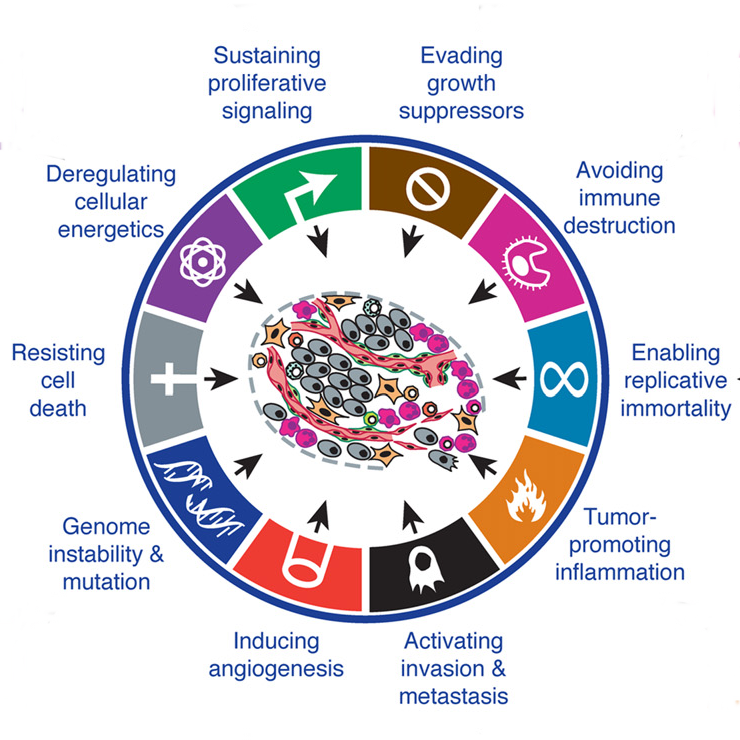
\includegraphics[width=0.8\linewidth]{intro/hallmarks}
	\caption[Hallmarks of Cancer]{Hallmarks of Cancer. The ten Hallmarks of Cancer as proposed by Hanahan and Weinberg in 2011. (Figure adapted from \citet{Hanahan2011})}
	\label{fig:hallmarks}
\end{figure}

\paragraph{Sustaining proliferative signalling}

\noindent
Cancer is a disease of uncontrolled cell proliferation and division.
However, without any external mitogenic growth signals, cancer cells cannot proliferate and therefore it is crucial for the cancer cells to maintain a steady proliferative signal.

There are many ways in which cancer cells can maintain this signal.
Firstly, cancer cells can acquire the ability to produce growth factors and express its corresponding receptor, creating a positive feedback mechanism that continuously stimulates the cells to proliferate \citep{Hanahan2000}.
Secondly, they can express more receptors for a given growth signals, and thus become ``hyperresponsive'' to the signal \citep{Hanahan2000,Hanahan2011}.
Thirdly, cancer cells can stimulate the neighbouring normal cells within its microenvironment to produce more growth factors that further assist them to grow \citep{Bhowmick2004, Liotta2001, Wiseman2002}.
Finally, cancer cells are able to maintain the proliferative signal by mutating the growth factor receptor itself, or the downstream signalling targets of the growth factor receptor pathway \citep{Fuqua1991,SuHuang1997,Satyamoorthy2003}.

By maintaining the the proliferative signals, cancer cells are able to continuously grow in their environment.

\paragraph{Evading growth suppressors}

\noindent
As well as maintaining proliferative signals, cancer cells must also evade the signals that inhibit cell growth.
Two tumour suppressor proteins have an essential role in this evasion: the \gls{rb} and p53 proteins.

\Gls{rb} protein is a known tumour suppressor protein that is important in cell cycle regulation \citep{Burkhart2008,Hanahan2011}.
\Gls{rb} protein is known to arrest the cells in \gls{g1} phase of the cell cycle by regulating E2F transcription factors in the cell, in reponse to molecules such as \gls{tgfb} \citep{Burkhart2008,Hanahan2000}.
Although \gls{rb} protein is known for its role as a checkpoint in \gls{g1} phase, it also takes part in the regulation of apoptotic cell death, cell differentiation and chromosome stability \citep{Burkhart2008}.
The contribution of the loss of function of the \gls{rb} protein in tumorigenesis and tumour progression is evident, but at which stage of the development this loss of function mutation is crucial for the cancer cells is yet to be clarified \citep{Burkhart2008}.

p53 protein is another tumour suppressor protein that is closely related to the \gls{rb} protein and its role in cell cycle arrest \citep{Hanahan2011,Levine1997}.
As \citet{Hanahan2011} mentions in their review, ``\gls{rb} transduces growth-inhibitory signals that originate largely outside of the cell, TP53 receives inputs from stress and abnormality sensors that function within the cell's intracellular operating systems''.
The level of expression and its stability is crucial for the function of p53 protein, as the abundance of p53 protein in the cell triggers cell cycle arrest or cell \gls{apoptosis}, depending on the extent of the cell signal \citep{Fridman2003,Hanahan2011,Levine1997}.
When abundant and active, p53 protein transcribes the p21 protein which, through series of events in the p16-cyclin D$_1$-cdk4-\gls{rb} pathway, triggers cell cycle arrest \citep{Levine1997}.

In many cancers, these proteins are usually mutated and selected against to allow continuous growth of the tumour cells.

\paragraph{Resisting cell death}

\noindent
\Gls{apoptosis}, the natural and controlled death of a cell, is one of many defence mechanisms in the body to prevent the development of cancer.
The triggering of \gls{apoptosis} is controlled and maintained by the balance between the pro- and anti-apoptotic signals that affect the downstream apoptotic proteins \citep{Hanahan2011}.

\Gls{bcl2} family proteins are the major players of apoptosis.
Embedded in the mitochondrial membrane, the Bax subfamily of \gls{bcl2} proteins are pro-apoptotic, and are under constant repression by the anti-apoptotic proteins of the \gls{bcl2} subfamily proteins \citep{Adams2007,Hanahan2011}.
The inhibition of the pro-apoptotic proteins are achieved by the interaction between the pro- and anti-apoptotic proteins via the \gls{bh3} domain \citep{Adams2007}.
In addition to the pro-apoptotic Bax subfamily proteins, there is a family of proteins that contain a single \gls{bh3} domain, and hence named \gls{bh3}-only family proteins \citep{Adams2007}.
\gls{bh3}-only proteins either disrupt the inhibition of the Bax family proteins by the \gls{bcl2} subfamily proteins, or directly stimulate the Bax subfamily proteins \citep{Adams2007}.
The activation of the pro-apoptotic proteins disrupt the mitochondrial cell membrane adn releases cytochrome \textit{c}, which in turn triggers the activation of the apoptotic proteases caspase 8 and caspase 9, resulting in apoptosis \citep{Adams2007,Hanahan2011}.

The precise cellular conditions that trigger apoptosis are yet to be uncovered, but there is a clear evidence of p53 tumour suppressor playing a key role in apoptosis initiation.
When \acrshort{dna} damage is sensed, p53 protein transcribes the pro-apoptotic members of the \gls{bcl2} family proteins, such as Bax, Puma and Noxa \citep{Fridman2003,Hanahan2011}.
The fact that p53 protein is involved not only in cell cycle regulation, but also in apoptotic pathway shows its importance in the control of cancer development, and perhaps that is the reason why more than 50\% of tumours have a mutation in the \textit{p53} gene \citep{Levine1997}.

\paragraph{Enabling replicative immortality}

\noindent
When acquired by cancer cells, the previous three hallmarks allow the cells to continuously grow in an uncontrolled manner.
However, this is not the case as the disruption in cell signalling on its own does not trigger the rapid expansion of the tumour -- only when the cells have the capability of replicating infinitely \citep{Hanahan2000, Hanahan2011}.

There are two barriers in achieving the infinite replicative capacity: senescence and crisis \citep{Hanahan2011}.
When cells are grown in a culture, cells are able to replicate and grow until a certain point, and the cells reach the stage of senescence where the cells stop growing but are still viable \citep{Hanahan2011}.
The cells that manage to bypass this senescence phase, by mutating the tumour suppressor proteins such as p53 and \gls{rb} proteins, then undergoes the crisis phase where the majority of the cells in the culture dies \citep{Hanahan2011}.
Very rarely, some cells are able to survive the crisis phase and acquires the ability to replicate infinitely, and this transition has been termed immortalisation \citep{Hanahan2011, Wright1989}.

Without immortalisation, cancer cells are not able to generate a macroscopic tumours that are capable of killing the host organism \citep{Hanahan2000,Hanahan2011}.

\paragraph{Inducing angiogenesis}

\noindent
Like normal cells, cancer cells also require access to oxygen and nutrient supply from the blood.
However, new blood vessel formation, or angiogenesis, only occurs in a handful of occasions, and thus the tumour needs to acquire the ability to stimulate angiogenesis in the microenvironment in which they live in \citep{Hanahan2011}.

It is thought that the angiogenic ability of the tumour is gained at an early stage of its development by disrupting the ``angiogenic switch'' \citep{Hanahan2011}.
Like many cellular processes, angiogenesis is controlled by the balance between the inducing and inhibiting agents of angiogenesis.
\Gls{vegfa} is the major growth factor that triggers angiogenesis by signalling through the \acrshort{vegf} receptors (though some receptors have inhibitory effect) \citep{Yancopoulos2000}.
Opposing the effect of \Gls{vegfa} is the \gls{tsp1}, a protein that is known to inhibit the process of angiogenesis by affecting the bioavailability of \acrshort{vegf}, as well as promoting apoptosis \citep{Kazerounian2008}.

In general, many cancers stimulate the expression of \gls{vegfa} protein and reduces the expression of \gls{tsp1} \citep{Kazerounian2008}.

\paragraph{Activating invasion and metastasis}

\noindent
One of the prime reasons that cancers are so difficult to treat and have high mortality is due to their ability to metastasise to other parts of the body.
Once metastasised to different parts of the body, the clinician not only has to consider the primary tumour site, but also the second, third, or even fourth tumour sites, which may or may not have similar tumour biology to the primary tumour, and thus have to consider multiple treatment plans to cure the patient.

Metastasis is a multi-step process that requires the selection and survival of cancer cell(s) that is able to metastasise (``seed''), and is also compatible with the specific target tissue where they prosper (``soil'') \citep{Talmadge2010}.
The downregulation or loss of function of E-cadherin, a protein important in cell-to-cell connection and adherence, is known to trigger tumour invasion and metastasis through the reversible process of \gls{emt} \citep{Hanahan2011,Kalluri2009}.
Once mobile and invasive, these metastatic cancer cell is able to circulate through the vascular system and eventually invade the target organ, where it must undergo \gls{met} and colonise the site \citep{Hanahan2011,Kalluri2009}.

There are numerous signals, growth factors and pathways that initiate the metastatic phenotype in cancer cell, and it remains an active field of research \citep{Hanahan2011,Kalluri2009}.

\paragraph{Genome instability and mutation}

\noindent
Many of the hallmarks are acquired by the cancer cells during its growth, through many genomic changes and mutations of the essential genes that allow cancer cells to survive, proliferate, invade and metastasise.
Thus, it is only logical to induce that many, if not all, cancers are more prone to genetic mutations and restructuring, which allows the cancers to subsequently acquire the already described Hallmarks of Cancer \citep{Hanahan2011}.

Until recently, the evolutionary progress of cancers have been thought to be gradual and stepwise, where each driver mutation is acquired over many years, or even decades \citep{Stephens2011}.
There are now evidence that show otherwise, whereby a single catastrophic event in the chromosome structure occurs, resulting in major structural rearrangements such as inversions, deletions, duplications and translocations \citep{Leibowitz2015,Stephens2011}.
This rare event that is estimated to occur in 2$\sim$5\% of all cancers was termed \gls{chromothripsis}, and is thought to be caused by the physical separation of parts of chromosome by a structure called micronuclei \citep{Leibowitz2015,Stephens2011}.
Owing to its nature of being a one-off chromosomal disruption, chromothripsis (usually) cause disruptions in tumour suppressor genes rather than duplications of oncogenes \citep{Leibowitz2015}.

In addition to this, areas of the chromosome where major structural rearrangements have occured can be prone to a regional hypermutation, termed \gls{kataegis} \citep{Leibowitz2015,Nik-Zainal2012}.
Although the full mechanism in which \gls{kataegis} occur is not yet defined, \gls{aid}/\acrshort{apobec} family proteins, a family of proteins involved in gene editing, may play a major role in \gls{kataegis} \citep{Leibowitz2015,Nik-Zainal2012}.
By deaminating cytidine to uracil in the \gls{ssdna} that may occur at the sites of double strand break, \gls{aid}/\acrshort{apobec} family proteins introduces hypermutated regions in the genome \citep{Leibowitz2015,Nik-Zainal2012}.

It is evident that both \gls{chromothripsis} and \gls{kataegis} contribute to the genomic aberrations and mutations that ultimately contribute to many of the tumorigenic phenotypes.

\paragraph{Tumour-promoting inflammation}

\noindent
Inflammation and immune response, though it may assist in the control of diseases and injuries, have been implicated in the progression of tumour and their acquisition of many of the hallmarks \citep{Hanahan2011}.

There are two pathways of inflammation that contribute to the cancer survival and progression \citep{Mantovani2008}.
The intrinsic pathway is caused by oncogenic characteristics of the cancer cells, where these cells produce inflammatory signals themselves and promote advantageous characteristics for the cancer cells, such as increased proliferation and survival \citep{Mantovani2008}.
On the other hand, the external pathway is caused by infectious or inflammatory conditions in the tumour microenvironment that surround the tumour and assist in the growth of the tumour \citep{Mantovani2008}.
There are two key transcription factors that connect these two pathways of inflammation that ultimately leads to the prommotion  of many, if not all, of the hallmarks discussed so far: \gls{nfkb} and \gls{stat3} \citep{Mantovani2008}.

The study by \citep{Pikarsky2004} showed that \gls{nfkb} was an essential component for the progression of hepatocellular carcinoma, providing the first evidence as to how inflammation may affect the tumour biology.
\gls{nfkb} regulates the expression of genes that encode the inflammatory cytokines, angiogenic factors, and many others, including anti-apoptotic genes (through the activation of \gls{stat3}) \citep{Elinav2013,Mantovani2008}.
\gls{stat3} is a transcription factor that is activated through variety of receptors and pathways, including the \gls{il6} receptor, \glspl{gpcr} and \glspl{tlr} \citep{Yu2007,Yu2014}.
By increasing the transcription of anti-apoptotic proteins such as \gls{bcl2}, \gls{stat3} promotes tumour survival and proliferation \citep{Yu2007}.
Furthermore, \gls{stat3} is able to increase the expression of inflammatory cytokines (such as \gls{il6} and \acrshort{il10}) and \acrshort{vegf}, which provides a positive feedback mechanism for further inflammation (and therefore survival and proliferation signals), and advancement of angiogenesis, respectively \citep{Yu2007}.

Though helpful at times, inflammation induced by the immune system must be taken care of and controlled in order to prevent rapid tumour development and progression.

\paragraph{Deregulating cellular energetics}

\noindent
In order to grow and proliferate, cancer cells must adjust their energy metabolism to match their energy requirement \citet{Hanahan2011}.
There are two ways in which a cell can produce energy: anaerobic respiration, where the cell uses glycolysis to rapidly generate \gls{atp} and lactate; and aerobic respiration where, in the presence of oxygen, the cell utilises the electron transport chain and \gls{atp} synthase in the mitochondria to efficiently produce \gls{atp}.
However, even with abundant oxygen in the cell, \citet{Wardburg1956} found that cancer cells utilised the glycolytic pathway instead of the more efficient aerobic respiration, which was later termed ``aerobic glycolysis'' \citep{Hanahan2011}.

It seems counterintuitive to limit its full potential of creating \gls{atp} by utilising glycolysis over electron transport chain, as the latter produces almost 18 times more \gls{atp} \citep{Hanahan2011, VanderHeiden2009}.
However, it is hypothesised  that this apprent inefficiency helps the cell to generate and direct the molecules required for biosynthetic pathways during cell growth and division \citep{Cairns2011,VanderHeiden2009}.
By deliberately relying purely on glycolysis (known as the ``Wardberg effect'') and slowing the conversion of \gls{pep} to pyruvate, the cell is able to shunt the carbon molecules into reaction pathways that produce constituents used to synthesise macromolecules, such as \acrshort{dna} and lipids \citep{Cairns2011,VanderHeiden2009}.

The fact that the deregulation of energy metabolism is mediated somewhat by the genes involved in many of the other hallmarks (such as p53 and Myc) suggests that the disruption in energy metabolism may be a phenotype caused in conjunction with those core hallmarks \citep{Hanahan2011}.

\paragraph{Avoiding immune destruction}

\noindent
Our immune system is constantly monitoring and maintaining normal cell biology within our body, preventing the emergence of cancer \citep{Hanahan2011}.
That said, cancers are frequently observed in clinics, pointing to the fact that the observed cancer cells must have evaded the diligent monitoring by the immune system \citep{Hanahan2011}.

Immunoediting is a process where the immune system successfully eliminates the highly immunogenic cancer cells during surveillance, but fails to eliminate the weakly immunogenic cells and therefore poses a selective advantage on these cells \citep{Hanahan2011,Teng2008}.
In fact, there has been reports where cancer cells in immunodeficient mice were not able to initiate tumour growth in the immunocompetent mice, but the cancer cells from the immunocompetent mice were able to do so in immunodeficient mice \citep{Hanahan2011}.
One possible reason for this was that the cancer cells from the immunodeficient mice were not immunoedited to the extent in which the cells from immunocompetent mice were, and thus unable to evade the immune system as efficiently as those cells in the immunocompetent mice \citep{Hanahan2011}.

Though more experiments must be carried out to confirm its definitive role and mechanisms in which it contributes to cancer biology, immune system evasion is in no doubt a significant component of tumour progression. \\

\noindent
By utilising many, if not all, of these major cancer hallmarks, cancer cells are able to initiate growth, proliferate, invade, metastasise and eventually kill the host if untreated.
There is an evident need for an efficient way to monitor and treat cancer patients, and these Hallmarks of Cancers will prove to be the best target for effective treatments of cancer in the future.


% TODO: do I really need tumour heterogeneity??
\subsubsection{Tumour heterogeneity (?)}
\label{subsub:tumour_heterogeneity}
TBC

\subsubsection{Cancer stem cells (?)}
\label{ssub:cancer_stem_cells}
TBC

\subsection{Causes and risk factors of cancer}
\label{sub:causes_and_risk_factors_of_cancer}

There are many causes and risk factors associated with the development and progression of cancer.
Like obesity, cancers are dependent on both the genetic and environmental factors.

\subsubsection{Genetic mutations}
\label{ssub:Genetic mutations}

It is quite obvious from the previous section (\cref{sub:mechanisms_of_cancer_development}: \nameref{sub:mechanisms_of_cancer_development}) that there are a lot of things that can go wrong in the cell.
Any one of the ten Hallmarks of Cancers has the potential to initiate cancer growth and progression; every hallmark has their own complex mechanistic pathways; every pathway has many proteins associated with its function or role in the cell; and, though their impacts may differ from protein to protein, mutations in any one of the proteins involved in a pathway has the potential to cause cancer.

% TODO: more citations!!!!
Broadly speaking, there are three major classes of genes that have significance in the initiation of cancer: oncogenes, tumour suppressor genes and stability genes \citep{Vogelstein2004a}.
Oncogenes are genes that promote or ``accelerate'' the process of tumorigenesis and/or tumour progression, whereas tumour suppressor genes prevent or ``decelerate'' those effects \citep{Vogelstein2004a}.
Cancers usually mutate the oncogenes in such a way that it it constitutively activated or expressed at a very high level, and mutate the tumour suppressor genes so that these genes are inactivated and/or have reduced expression \citep{Vogelstein2004a}.
Another thing to note for these genes is that oncogenes usually only require a ``one-hit'' mutation that affects a single allele, whereas tumour suppressor genes require mutations in both maternal and paternal alleles to have any effect \citep{Stratton2009,Vogelstein2004a}.

Stability genes, also known as caretakers, are genes that are involved in, for example,  \gls{mmr}, \gls{ner} and \gls{ber}; in other words, genes that are involved in \acrshort{dna} repair mechanisms \citep{Vogelstein2004a}.
These caretaker genes in effect prevents the cell to develop new mutations from \acrshort{dna} replication and mitosis.
However, only the oncogenes or the tumour suppressor genes are able to directly affect the biology of the cell, and therefore mutations in the stability genes affect the mutation rates of the other classes of genes, ultimately leading to tumorigenesis \citep{Vogelstein2004a}.
\\

\noindent
There are two types of mutations that occurs in an individual: germline mutation and somatic mutation.
Germline mutations are the mutations that are passed on from your parents, and somatic mutations are the mutations acquired by the cell over the course of the individual's lifetime.

Unfortunately, there are germline mutations that make the individual more prediposed to cancer \citep{Vogelstein2004a}.
These individuals have a mutation in one or more of the classes of cancer-related genes, which makes them more likely to develop tumour than their normal pairs \citep{Vogelstein2004a}.
As a consequence, these individuals may develop multiple tumours at an early stage of their lives than those who develop tumours from somatic mutations alone, as these individuals already have a mutation that allows all of the cells in their body to have one or more of the Hallmarks of Cancers \citep{Vogelstein2004a}.

In contrast, somatic mutations are acquired during an individual's lifetime and is not passed down to their children.
Somatic mutations can either be a driver or a passenger mutation, where a driver mutation helps tumorigenesis and its subsequent progression (in other words, mutations in oncogene, tumour suppressor, or stability gene), and passenger mutation is where the mutation has no selective advantage for the cancer and does not contribute to tumour progression \citep{Stratton2009}.
Since cancers require multiple driver mutations, somatic mutations are an essential part of tumour development.
Perhaps that is one of the reasons why, in some cancers, germline mutation in the stability genes cause greater susceptibility to cancers than mutations in oncogene or tumour suppressor gene \citep{Vogelstein2004a}.

\subsubsection{Environmental factors}
\label{ssub:environmental_factors}

For obesity, since there is a clear evidence of the cause (excessive eating and lack of exercise) and a well defined mechanism of how the disease is developed (excess calories are converted into fat), it is relatively easy to speculate the effect of the environment on the disease (for example, abundance of high calory food).
On the other hand, cancers are developed through many cellular pathways (Hallmarks of Cancers) which are not fully uncovered yet, with either too many or very few causes associated with those pathways (for example, mutations, inflammation and/or growth factors), and therefore it is difficult to assess how, rather than whether, a given environmental factor causes specific cancer.

With that said, there has been a few environmental factors that have a strong evidence of causing cancer, though the complete mechanism of action for some of these must be elucidated in the coming years.
Out of these, smoking, \gls{uv} radiation, and diet and obesity will be covered as examples.
\\

% Smoking
\noindent
Smoking is a known risk factor for many cancers; the obvious one being lung cancer \citep{Gandini2008,Hecht1999}.
For current smokers, the relative risk is greater than 1.5 in many cancers, including liver, cervix and kidney, and it can rise up to 8.96 in lung cancer \citep{Gandini2008}.
Even if smokers stop smoking, the relative risk does not decrease until the first 5 years have passed and will never return to the level of non-smokers \citep{Hecht1999}.

In tobacco smoke, there are literally hundreds and thousands of chemical compounds, of which about 20 compounds have been shown to have carcinogenic effects \citep{Hecht1999}.
Among these, \glspl{pah} and \gls{nnk} have been shown to cause lung cancer in mice when administered systemically \citep{Hecht1999}.
These carcinogens are processed first by \gls{cyp} enzymes (termed meta\-bolic activation), and the product can either be processed further to be detoxified completely and cause no harm to the cell, or alternatively, the product can covalently bind to the \acrshort{dna}, forming \acrshort{dna} adducts \citep{Hecht1999}.
Unless these adducts are resolved correctly by the \acrshort{dna} repair mechanisms, it can result in a permanent mutation within the genome and lead to oncogenesis \citep{Hecht1999}.

In addition to this, cigarettes contain free radicals and chemicals that cause tremendous oxidative stress and damage to the cells \citep{Hecht1999}.
These radicals cause \acrshort{dna} nicks and damages the \acrshort{dna}, again requring the cell's \acrshort{dna} repair mechanisms to remove the damage so it does not become permanent.
\\

% UV radiation
\noindent
Another important environmental factor to consider is \gls{uv} radiation.
Exposure to \gls{uv} radiation has been significantly associated with the increased risks of skin cancers \citep{Armstrong2001,Gallagher2006}.
The risks of developing any skin cancers can vary between race (Caucasian people are more likely to get skin cancers), and potentially the age when they were exposed to high amounts of \gls{uv} radiation \citep{Armstrong2001,Gallagher2006}.

Again, the mechanism of how \gls{uv} radiation may cause  skin cancers is related to the \acrshort{dna} repair system.
\gls{uv} radiation causes the formation of a dimer in the adjacent pyrimidines, resulting in a covalent bond formation between these nucleotides \citep{Friedberg2003,Hoeijmakers2001}.
These dimers introduce bulky structures in the \acrshort{dna} that prevent the \acrshort{dna} replication and transcription enzymes from functioning properly, and if they are not repaired, it may cause lasting mutations \citep{Friedberg2003,Hoeijmakers2001}.
These damages caused by \gls{uv} radiation can be relieved by the \gls{ner} system or the photoreactivation process, where a photoreactivating enzyme uses light to monomerize the dimeric pyrimidines \citep{Friedberg2003}.
\\

% Diet and obesity
\noindent
Finally, diet and obesity are known risk factors for many types of cancers \citep{Ames1995a,Calle2004}.
Though more will be covered in details in \cref{sec:obesity_and_cancers}: \nameref{sec:obesity_and_cancers}, the effect of obesity on cancers will be briefly mentioned here.

Epidemiological evidence of obesity being a risk factor for many cancers has been well established, yet the mechanisms of its contribution to cancer is still  speculative \citep{Calle2003,Kelesidis2006a}.
Although there are a lot of possible mechcanisms, there is growing evidence of the role of chronic inflammation caused by increased fat mass in the body \citep{Kelesidis2006a,Lumeng2011,Hernandez2013}.
Free fatty acids from excess adipose tissue and/or diet can be recognised by the \gls{tlr}4, which can then activate \gls{nfkb} \citep{Lumeng2011}.
Clearly, the result of the activation of \gls{nfkb} can lead to the activation of one of the Hallmarks of Cancers -- tumour-promoting inflammation.

The nutritional content of the food that people consume is also important, as it can both directly and indirectly influence the likelihood of tumorigenesis, as well as its progression \citep{Ames1995a}.
Many fruits and vegetables contain antioxidants as well as essential viatmins and minerals.
Antioxidants are able to neutralise the effect of \gls{ros},  and many viatmins have been associated with reduction of many types of cancers \citep{Ames1995a}.
In fact, ascorbic acid (vitamin C) is able to prevent the lipid peroxidation of lipid plasma caused by tobacco smokes \textit{in vitro}, which could be why smokers, compared to non-smokers, have decreased levels of ascorbic acid \citep{Hecht1999}.

By maintaining healthy diet, it may be possible to reduce the risks of many cancers and obesity, as well as the comorbidities associated with them.
\\

\noindent
As one can imagine, \acrshort{dna} damages caused by smoking and/or \gls{uv} radiation have the potential to damage the genome and initiate cancer if wrong genes are mutated, such as p53 tumour suppressor gene.
Healthy diet is also crucial for lowering the risk of cancers through beneficial vitamins and antioxidants, and prevent obesity as well as chronic inflammation that accompanies with it.
There are many other environmental factors associated with cancers, and limiting the exposure to detrimental environmental factors is crucial for the prevention of any types of cancers, as well as the more specific types of cancers associated with these factors, such as lung and skin cancers.
\\

\subsection{Treatment of cancer}
\label{sub:treatment_of_cancer}

Traditionally, the treatment of cancer has been surgery, radiation therapy and chemotherapy.
Though surgery is an effective method to remove the tumour from the patient, there is always a risk of metastasis and recurrence, which is why combination of surgery with other treatments like chemotherapy is usually considered.
Earlier chemotherapeutic drugs and radiation therapy had limited effect on tumours due to their resistance against these treatments \citep{Wilhelm2006}.
However, greater understanding of the pathways and mechanisms that tumour cells use have shed  light on the development of drugs that are more effective against tumours.
RAF inhibitors are among one of many.

The RAS-RAF-MEK-ERK signalling pathway is a pathway involved in cell survival, growth and proliferation \citep{Samatar2014,Wilhelm2006}.
The members of this pathway are often mutated in many types of cancers, causing an overactivation of this pathway.
For example, approximately a third of cancers contain a mutation in the RAS oncogene which allows the constitutive activation of the RAS-ERK pathway \citep{Samatar2014}.
Development of the drugs that target  the downstream RAF and its mutant forms (such as BRAF$^{V600E}$) have been successful, and many RAF inhibitor drugs such as sorafenib and vemurafenib have been approved for use clinically \citep{Samatar2014,Wilhelm2006}.
Even though our understandings of signalling pathways and drug development based on these knowledge is improving, there is always the possibility of tumour to acquire resistance to those drugs and there is always a need for new ways to treat cancer patients \citep{Samatar2014}.

In fact, there has been evidence of pathway cross-talks between RAS-ERK pathway and \gls{pi3k}/Akt pathway \citep{Moelling2002,Zimmermann1999a}.
Furthermore, a study in \textit{Drosophila} showed that the inhibition of just a single pathway does not necessarily stop the effect of the pathway, as the signal can flow through alternate pathways \citep{Dar2012}.
Pathway cross-talk and increased flux through alternate pathways could be one of the ways in which tumour cells acquire resistance to drugs.
However, the effectiveness of targeting multiple pathways in humans is yet to be confirmed and further investigations are required to solidify the mode of action and its relevance to tumour biology.
\\

\noindent
Though there are difficulties such as resistance to drugs and metastasis, further development of technologies and improved knowledge of tumour biology will only get us closer to the cure of cancer.

\section{Obesity and cancers}
\label{sec:obesity_and_cancers}

As mentioned briefly in \cref{sub:causes_and_risk_factors_of_cancer}: \nameref{sub:causes_and_risk_factors_of_cancer}, obesity is considered a major risk factor for many types of cancers.
The fact that the prevalence of obesity is extremely high, it is important to establish the link between the apparent risks associated with cancer.

\subsection{Cancer risks associated with obesity}
\label{sub:cancer_risks_associated_with_obesity}

Although the mechanisms in which obesity causes cancer is still under debate, the association between obesity and cancer has long been established.

Perhaps the most convincing evidence of the association between obesity and cancer was first presented by \citet{Calle2003}.
In this study, the link between \gls{bmi} and variety of cancers were investigated in 900,000 adults between 1982 and 1998 \citep{Calle2003}.
The results from this study showed that morbidly obese men and women (\gls{bmi} \textgreater{} 40) had 52\% and 62\% higher chance of dying from all cancers compared to normal weight adults (18.5 \textgreater{} \gls{bmi} \textgreater{} 25), respectively \citep{Calle2003}.
\gls{bmi} was also associated with higher rates of death from esophageal, colorectal, liver, gallbladder, pancreas, kidney, and some sex-specific cancers \citep{Calle2003}.
Furthermore, the death rates had a positive linear correlation with increasing \gls{bmi} in all cancers \citep{Calle2003}.

In a more recent meta-analysis study by \citet{Renehan2008} showed that an increase \gls{bmi} by 5 kg/m$^2$ significantly increased the risks of esophageal, thyroid, colon and renal cancers in men; endometrial, gallbladder, esophageal and renal cancers in women.
The summary of the risks associated with various cancers from this study are shown in \cref{tab:renehan_cancer_risks}.
This study showed that the association between \gls{bmi} and cancers were sex-specific, applicable to wide range of cancer types, and generally consistent across geographic populations \citep{Renehan2008,Roberts2010}.

Taken together, it is undeniable that obesity is a major risk factor for many types of cancers, and it may even be the cause for some of these cancers.

\begin{table}[h]
	\centering
	\begin{threeparttable}
		\caption{Summary of the risk ratios\tnote{1} that significantly associated with each cancer types from \citet{Renehan2008} study\tnote{2}.}
		\label{tab:renehan_cancer_risks}
		\begin{tabular}{lcc}
													   & Men               & Women\\
			\hline
			\rule{0pt}{2.25ex}Colon                 & 1.24 (1.20, 1.28) & 1.09 (1.05, 1.13)\\
			Rectum                                  & 1.09 (1.06, 1.12) & NA\tnote{3}\\
			Gallbladder                             & NA                & 1.59 (1.02, 2.47)\\
			Leukemia                                & 1.08 (1.02, 1.14) & 1.17 (1.04, 1.32)\\
			Malignant melanoma                      & 1.17 (1.05, 1.30) & NA\\
			Multiple myeloma                        & 1.11 (1.05, 1.18) & 1.11 (1.07, 1.15)\\
			Non-Hodgkin lymphoma                    & 1.06 (1.03, 1.09) & 1.07 (1.00, 1.14)\\
			Esophageal adenocarcinoma               & 1.52 (1.33, 1.74) & 1.51 (1.31, 1.74)\\
			Pancreatic                              & NA                & 1.12 (1.02, 1.22)\\
			Renal                                   & 1.24 (1.15, 1.34) & 1.34 (1.25, 1.43)\\
			Thyroid                                 & 1.33 (1.04, 1.70) & 1.14 (1.06, 1.23)\\
			Prostate                                & 1.03 (1.00, 1.09) & NA\\
			Post-menopausal breast                  & NA                & 1.12 (1.08, 1.16)\\
			Endometrial (\textless{}27 kg/m$^2$)    & NA                & 1.221 (1.084, 1.376)\\
			Endometrial (\textgreater{}27 kg/m$^2$) & NA                & 1.729 (1.598, 1.872)\\
		\end{tabular}
		\begin{tablenotes}
			\begin{footnotesize}
				\item [1] All risk ratios are per increase in 5 kg/m$^2$ \gls{bmi}.
				\item [2] This table is adapted from \citet{Roberts2010} paper, where the original data is taken from \citet{Renehan2008} paper.
				\item [3] Not applicable.
			\end{footnotesize}
		\end{tablenotes}
	\end{threeparttable}
\end{table}

\subsection{Mechanism of cancer progression in obese patient}
\label{sub:mechanism_of_cancer_progression_in_obese_patient}

% Why is it important in obesity context.

% The exact mechanism in which obesity accelerates cancer progression is unknown, but obesity is thought to disrupt the levels of various hormones (such as insulin, leptin, adeponectin, and other adipokines) that eventually activate tumorigenic pathways (reference the overview on obesity and tumour resistance).









\section{Genetic signatures}
\label{sec:genetic_signatures}

\subsection{Microarray and Next Generation Sequencing technologies}
\label{sub:microarray_and_next_generation_sequencing_technologies}

% Due to advances in sequencing technology over the last few years, many researchers have started to focus on bioinformatics based analyses of cancer cells to better understand the biology of cancer.
% Advantages of this strategy are that very specific gene expression and/or mutational signatures for certain cancer subtypes can be identified from the analyses, which the researchers and clinicians can study in much greater depth and details.

\subsection{Obesity associated genetic signatures}
\label{sub:obesity_associated_genetic_signatures}

\subsubsection{\citet{Creighton2012} study}
\label{ssub:creighton_study}



\subsubsection{\citet{Fuentes-Mattei2014} study}
\label{ssub:fuentes_mattei_study}




\subsection{Pathway associated genetic signatures}
\label{sub:pathway_associated_genetic_signatures}

% Talk about \citet{Gatza2010a}

\subsubsection{\citet{Gatza2011} study}
\label{ssub:gatza_study}





\section{Aim of the project}
\label{sec:aim}

This research aims to determine whether gene expression signatures exist  that are specific to obesity across multiple cancer types, and to investigate whether there are any common pathways being dysregulated in cancers based on these genetic signatures.
Better understanding of the pathways being dysregulated in cancer cells in obese patients may lead to improved clinical decisions, and contribute towards personalised treatment in the future.

